% !TeX spellcheck = si_SI
\chapter{Implementacija rešitve}\label{cha:rezultati}

Naloga je torej ustvariti vmesno vozlišče v ROS-u, ki jemlje podatke o obstoječi poti iz navigacijskega algoritma ter jih ustrezno transformira ter pošilja naslednjemu vozlišču, ki je odgovoren za izvajanje sledenja novo ustvarjeni poti. Pri določanju območja glajenja se bo upoštevala tudi prisotnost ovir, zato bo potrebno brati tudi informacije o zemljevidu vrednosti. Za implementacijo rešitve je najprej potrebno ustvariti razvojno okolje.

\section{Priprava razvojnega okolja}

Omenjeno vozilo v razvoju ni bilo lahko razpoložljivo, na srečo nam ROS paket nudi povezljivost s simulacijskim okoljem Gazebo. Gazebo je odprtokodno simulacijsko okolje za testiranje robotov, ki nudi dinamske simulacije, 3D prikaz, generacijo poljubnega modela robota in okolja in še marsikaj drugega. Omenjeni program smo uporabljali v kombinaciji z ROS paketom RViz, ki nudi 3D prikaz robota, okolja ter prikaz vseh vrst senzorksih podatkov, kot so na primer točke zajete pridobljene z lidar-jem. Najpomembnejše je to, da nam RViz prikazuje podatke o poti, ki jo nudi navigacijski algoritem in tako nudi takojšnjo preverbo. Da okolje izpopolnimo, potrebujemo še testno vozilo. Uporabili smo paket, ki ga nudi spletni blog moorerobots \cite{vir10}, ta vsebuje preprosto vozilo z diferencialnim pogonom in prirejeno realizacijo navgiacijskega algoritma. Delali bomo z ROS izvedbo Kinetic Kame na operacijskem sistemu Linux Ubuntu. Z definiranim okoljem sedaj lahko začnemo na razvoju omenjenega vozlišča vokolju ROS.

\section{ROS vozlišče}

\subsection{Pomembnejše povezave vozlišča}


Za navigacijo robota v okolju ROS skrbi tako imenovani navigacijski sklad (ang. \textit{Navigation Stack}), katerega bistveno vozlišče se imenuje \texttt{/move\_base}. To vozlišče na podlagi podane ciljne točke, zemljevida okolice in bližnje okolice zaznane z laserskim merilnikom ustvari globalen načrt oziroma pot ter lokalno pot, katere namen je, da skuša vozilo karseda približati globalni. Glajena bo pot globalnega načrta, ki jo \texttt{/move\_base} pošilja po komunikacijski povezavi (\textit{Topic}) \texttt{/move\_base/TrajectoryPlannerROS/global\_plan}. \newline Sporočila te povezave so tipa \texttt{nav\_msgs/Path} in nosijo informacijo o legah točk poti ter o orientaciji v ciljni točki. Ker se pri določanju območja glajenja upošteva tudi prisotnost ovir oziroma zemljevid vrednosti je potrebno brati tudi sporočila tipa \newline \texttt{nav\_msgs/OccupancyGrid}, ki jih navigacijski sklad pošilja po povezavi \newline \texttt{/move\_base/global\_costmap/costmap}. Lega ovir se s časom lahko spreminja zato se tudi zemljevid vrednosti s časom spremija in posledično je potrebno njegovo informacijo dopolnjevati s sporočila tipa \texttt{map\_msgs/OccupancyGridUpdate}, ki jih dobimo preko kanala
\texttt{/move\_base/global\_costmap/costmap\_updates}.

\subsection{Delovanje vozlišča}

Vozlišče je zasnovano tako, da ima zavoljo enostavnosti uporabe avtomatizirano nastavljanje pramaterov ob njegovem zagonu. Ideja je realizirana tako, da vozlišče deluje kot avtomat (ang. \textit{State Machine}) z dvemi stanji. Naloga prvega stanja je nastavitev prametrov, naloga drugega pa je glajenje poti po tem ko so paramteri glajenja ugotovljeni.

\subsubsection{Iskanje parametrov}

Iskanje paramterov je izvedeno tako, da se ob zagonu vozlišča glajenja, ki smo ga poimenovali \texttt{/path\_smoothing\_node} vozlišču \texttt{/move\_base} pošilja naključne cilje z ozirom na zemljevid vrednosti (če je cilj podan na mesto ovire nam navigacijski sklad ne ustvari poti). Namen tega je pridobitev ustrezno grobe poti na podlagi katere izvedemo optimizacijo s katero iščemo optimalne parametre. Ustreznost poti na kateri temelji optimizacija ocenimo na podlagi srednje vrednosti in standardne deviacije absolutne vrednosti kotov med posameznimi daljicami, ki tvorijo grobo pot.

Ko je ustrezna pot najdena začenmo z iskanjem minimuma kriterijske funkcije, ki je definirana kot srednja vrednost absolutnih kotov med odseki poti. Metoda iskanja ekstrema je Nelder-Mead, ki deluje na sledeč način. Pri tej metodi iščemo ekstrem funkcije z uporabo tako imenovanega simplexa. To je $n+1$ dimenzionalen enakostraničen politop v $n$ parametrskem prostoru (Slika \ref{fig:slika6}, primer a). V našem primeru optimiramo dva paramtera (masa in dušenje) zato je simplex enakostraničen trikotnik.

\begin{figure}[H]
	\centering
	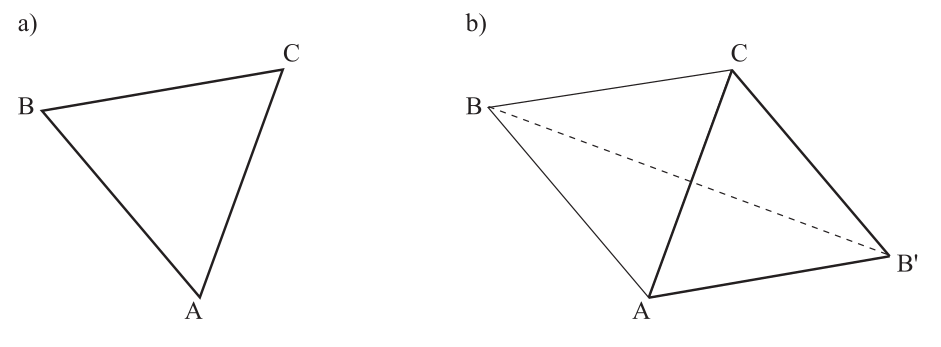
\includegraphics[width=10cm]{pic/simplex.png}
	\caption{Simplex \cite{vir11}.}
	\label{fig:slika6}
\end{figure}

Prvi korak iskanja minimuma funkcije s simplexom je tvorba simplexa na podlagi začetnih približkov \cite{vir11}. Nato se najde točko na simplexu, ki vrne največjo vrednost kriterijske funkcije. To točko se nato preslika preko lika tako, da tvorimo nov simplex (Slika \ref{fig:slika6}, primer b). Postopek ponavljamo toliko časa, dokler ne konvergiramo v okolico lokalnega minimuma.

Prednost metode je v tem, da ne potrebujemo matematično definirane kriterijske funckije (lahko je funkcija v programskem smislu) in posledičnega odvoda, ki ga za razliko od te metode potrebujejo gradientne metode. V našem primeru smo uporabili več začenih približkov z namenom bolj globalnega preiskovanja kriterijske funckije. Ko so z omenjenim pristopom najedni optimalni paramteri jih uporabimo v naslednjem stanju avtomata, ki predstavlja jedro vozlišča. Prvo stanje v vozlišče vnaša nekaj ROS paramterov, ki jih lahko nadziramo s paketom \texttt{dynamic\_reconfigure}. Ti parametri so značilke na podlagi kerih iščemo grobo pot, to so torej srednja vrednost, standardna deviacija absolutnih kotov ter minimalna dolžina poti. Ko je nova pot pridobljena sledi še njena objava.

\subsubsection{Glajenje poti}

Jedro vozlišča, ki ga predstavlja glajenje poti je sestavljeno iz petih ključnih funkcij, ki so realizirane v programskem jeziku Python. Naloga prve funckije je branje obstoječe grobe poti, ki jo vrača navigacijski sklad. Prva funckija vrne grobo pot v urejeni obliki 2D polja točk. To polje točk nato prevzame druga funckija, ki doda vmesne točke, kar poveča učinek algoritma glajenja. Na podlagi polja z dodanimi točkami ter zemljevida vrednosti se v tretji funkciji določa območje glajenja. Cilj te funkcije je določiti območje glajenja z ozirom na zemljevid vrednosti, to pa se izvede tako, da se skozi točke poti v pravokotni smeri inkrementalno premikamo vzdolž normale ter preverjamo pripadajoče mesto v zemljevidu vrednosti. Preverjanje zemljevida vrednosti je izvedeno tako, da se inkrementirano točko pretvori v element matrike, ki predstavlja realizacijo zemljevida vrednosti in preveri vrednost omenjenega elementa. Ko dosežemo oviro ozrioma mejo inkremetiranja se postopek ustavi, dosežena razdalja pa se doda v polje razdalj od poti do ovire. Postopek se ponavlja za vsako točko poti na levi in desni strani glede na pot, tako dobimo dve polji (levo in desno) razdalj od poti do ovire. Primer območja v oklici poti lahko vidimo na sliki \ref{fig:slika_obm}, kjer rdeči linji predstavljata meji območja, modra linija pa grobo pot. Na sliki \ref{fig:slika_obm} črna polja predstavljajo prisotnost ovire. Polje točk grobe poti ter polji, ki tvorita območje galjenja se nato uporabi v funkciji s katero gladimo pot na način, ki je opisan v poglavju 5. Pri tem uporabimo paramtere ugotovljene v prvem stanju algoritma. Ostali paramteri glajenja so število iteracij s katerimi določamo lego po enačbi \ref{eq:16}, korak inkrementalnega preverjanja območja glajenja, meja inkrementiranja ter prag vrednosti ovire v zemljevidu vrednosti. Ko je pot zglajena sledi njena objava v sporočilu oblike \verb|/nav_msgs/Path|, ki vsebuje točke poti ter orientacijo v zadnji točki.

\begin{figure}[H]
	\centering
	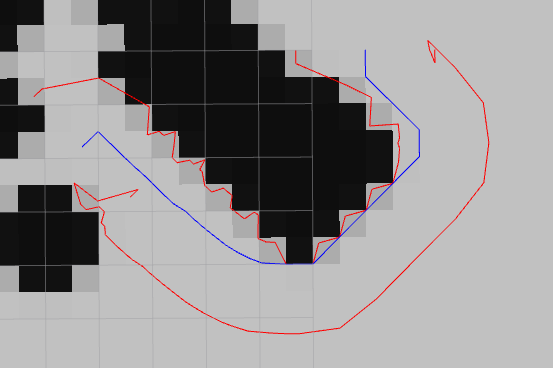
\includegraphics[width=10cm]{pic/obmocje.png}
	\caption{Primer določanja območja glajenja v programu RViz.}
	\label{fig:slika_obm}
\end{figure}


\begin{figure}[H]
	\centering
	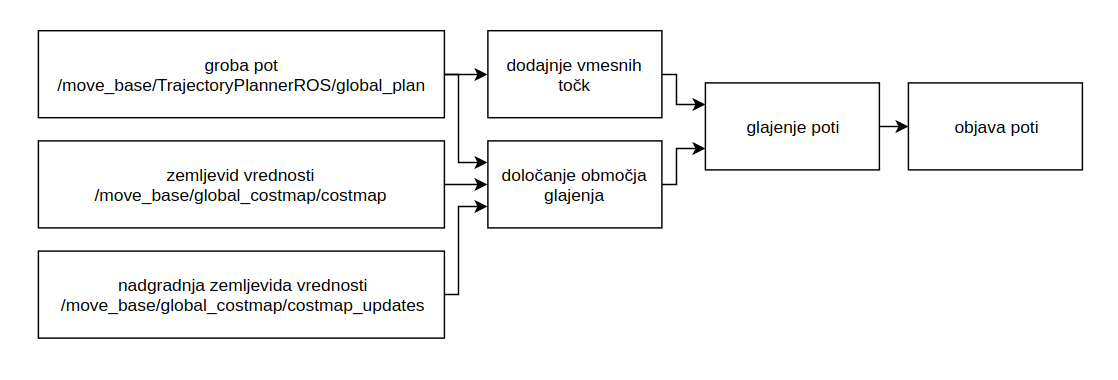
\includegraphics[width=16cm]{pic/shema.png}
	\caption{Shema delovanja algoritma glajenja poti.}
	\label{fig:slika6}
\end{figure}
